\documentclass[]{article}
\usepackage{lmodern}
\usepackage{amssymb,amsmath}
\usepackage{ifxetex,ifluatex}
\usepackage{fixltx2e} % provides \textsubscript
\ifnum 0\ifxetex 1\fi\ifluatex 1\fi=0 % if pdftex
  \usepackage[T1]{fontenc}
  \usepackage[utf8]{inputenc}
\else % if luatex or xelatex
  \ifxetex
    \usepackage{mathspec}
  \else
    \usepackage{fontspec}
  \fi
  \defaultfontfeatures{Ligatures=TeX,Scale=MatchLowercase}
\fi
% use upquote if available, for straight quotes in verbatim environments
\IfFileExists{upquote.sty}{\usepackage{upquote}}{}
% use microtype if available
\IfFileExists{microtype.sty}{%
\usepackage{microtype}
\UseMicrotypeSet[protrusion]{basicmath} % disable protrusion for tt fonts
}{}
\usepackage[margin=1in]{geometry}
\usepackage{hyperref}
\PassOptionsToPackage{usenames,dvipsnames}{color} % color is loaded by hyperref
\hypersetup{unicode=true,
            pdftitle={DSCI354-451 Foundation : Inference, EDA, DSCI Process},
            pdfauthor={Roger H. French, JiQi Liu},
            colorlinks=true,
            linkcolor=Maroon,
            citecolor=Blue,
            urlcolor=blue,
            breaklinks=true}
\urlstyle{same}  % don't use monospace font for urls
\usepackage{graphicx,grffile}
\makeatletter
\def\maxwidth{\ifdim\Gin@nat@width>\linewidth\linewidth\else\Gin@nat@width\fi}
\def\maxheight{\ifdim\Gin@nat@height>\textheight\textheight\else\Gin@nat@height\fi}
\makeatother
% Scale images if necessary, so that they will not overflow the page
% margins by default, and it is still possible to overwrite the defaults
% using explicit options in \includegraphics[width, height, ...]{}
\setkeys{Gin}{width=\maxwidth,height=\maxheight,keepaspectratio}
\IfFileExists{parskip.sty}{%
\usepackage{parskip}
}{% else
\setlength{\parindent}{0pt}
\setlength{\parskip}{6pt plus 2pt minus 1pt}
}
\setlength{\emergencystretch}{3em}  % prevent overfull lines
\providecommand{\tightlist}{%
  \setlength{\itemsep}{0pt}\setlength{\parskip}{0pt}}
\setcounter{secnumdepth}{5}
% Redefines (sub)paragraphs to behave more like sections
\ifx\paragraph\undefined\else
\let\oldparagraph\paragraph
\renewcommand{\paragraph}[1]{\oldparagraph{#1}\mbox{}}
\fi
\ifx\subparagraph\undefined\else
\let\oldsubparagraph\subparagraph
\renewcommand{\subparagraph}[1]{\oldsubparagraph{#1}\mbox{}}
\fi

%%% Use protect on footnotes to avoid problems with footnotes in titles
\let\rmarkdownfootnote\footnote%
\def\footnote{\protect\rmarkdownfootnote}

%%% Change title format to be more compact
\usepackage{titling}

% Create subtitle command for use in maketitle
\newcommand{\subtitle}[1]{
  \posttitle{
    \begin{center}\large#1\end{center}
    }
}

\setlength{\droptitle}{-2em}

  \title{DSCI354-451 Foundation : Inference, EDA, DSCI Process}
    \pretitle{\vspace{\droptitle}\centering\huge}
  \posttitle{\par}
    \author{Roger H. French, JiQi Liu}
    \preauthor{\centering\large\emph}
  \postauthor{\par}
      \predate{\centering\large\emph}
  \postdate{\par}
    \date{29 September, 2018}


\begin{document}
\maketitle

{
\hypersetup{linkcolor=black}
\setcounter{tocdepth}{6}
\tableofcontents
}
\setcounter{section}{6} \setcounter{subsection}{1}
\setcounter{subsubsection}{0}

\paragraph{Reading, Homeworks, Projects,
SemProjects}\label{reading-homeworks-projects-semprojects}

\begin{itemize}
\tightlist
\item
  MidTerm Exam next Thursday October 11th

  \begin{itemize}
  \tightlist
  \item
    MidTerm Review in class Tuesday October 9th
  \end{itemize}
\item
  Readings:

  \begin{itemize}
  \tightlist
  \item
    R4DS 9-16 Data Wrangling for today
  \end{itemize}
\item
  Homeworks

  \begin{itemize}
  \tightlist
  \item
    HW4 given out next Thursday Oct. 12th
  \item
    Due following Tuesday October 17th
  \end{itemize}
\item
  Data Science Projects:

  \begin{itemize}
  \item
  \end{itemize}
\item
  451 SemProjects:

  \begin{itemize}
  \item
  \end{itemize}
\item
  Friday Comm. Hour

  \begin{itemize}
  \item
  \end{itemize}
\end{itemize}

\paragraph{Textbooks}\label{textbooks}

\begin{itemize}
\tightlist
\item
  \href{https://play.google.com/books/reader?printsec=frontcover\&output=reader\&id=F1mVHgAAAEAJ\&pg=GBS.PA1}{Peng:
  R Programming for Data Science}
\item
  \href{https://play.google.com/books/reader?printsec=frontcover\&output=reader\&id=R-09BgAAAEAJ\&pg=GBS.PA1}{Peng:
  Exploratory Data Analysis with R}
\item
  \href{https://play.google.com/books/reader?printsec=frontcover\&output=reader\&id=G2EOBwAAAEAJ\&pg=GBS.PA0}{Open
  Intro Stats, v3}
\item
  \href{https://play.google.com/books/reader?printsec=frontcover\&output=reader\&id=I6y3DQAAQBAJ\&pg=GBS.PA1}{Wickham:
  R for Data Science}
\item
  \href{https://play.google.com/books/reader?printsec=frontcover\&output=reader\&id=KtuPCwAAAEAJ\&pg=GBS.PA0}{Hastie:
  Intro to Statistical Learning with R}
\end{itemize}

\paragraph{Syllabus}\label{syllabus}

\begin{figure}
\centering
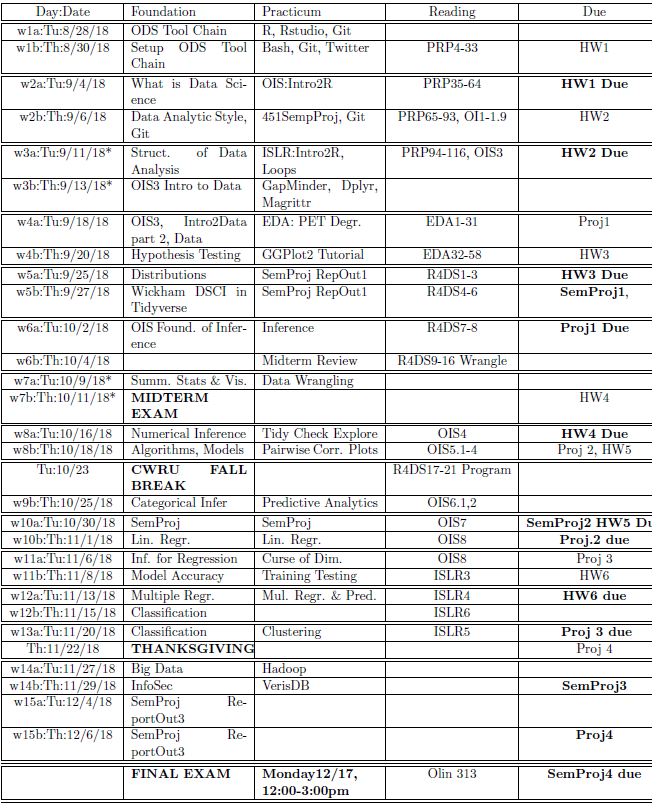
\includegraphics{./figs/syllabus.png}
\caption{DSCI351-451 Syllabus}
\end{figure}

\paragraph{Statistical Inference, Exploratory Data Analysis, and the
Data Science
Process}\label{statistical-inference-exploratory-data-analysis-and-the-data-science-process}

\subparagraph{Doing Data Science}\label{doing-data-science}

\begin{itemize}
\tightlist
\item
  What to be thinking about as we do DSCI
\end{itemize}

\subparagraph{Statistical Thinking in the Age of Big
Data}\label{statistical-thinking-in-the-age-of-big-data}

\href{http://www.nytimes.com/2012/02/12/sunday-review/big-datas-impact-in-the-world.html?mcubz=1}{The
Age of Big Data, Steve Lohr, The New York Times}

Big Data is a vague term, used loosely, if often, these days. But put
simply, the catchall phrase means three things.

\begin{itemize}
\tightlist
\item
  First, it is a bundle of technologies.
\item
  Second, it is a potential revolution in measurement.
\item
  And third, it is a point of view, or philosophy,

  \begin{itemize}
  \tightlist
  \item
    about how decisions will be---and perhaps should be---made in the
    future.
  \end{itemize}
\end{itemize}

Data Science is a practical mixture of Statistics, Coding, Linear
Algebra,

\begin{itemize}
\tightlist
\item
  And Domain Knowledge
\end{itemize}

\paragraph{Frequentist vs.~Bayesian
Statistics}\label{frequentist-vs.bayesian-statistics}

\subparagraph{Frequentist Statistics has to do
with}\label{frequentist-statistics-has-to-do-with}

\begin{itemize}
\tightlist
\item
  Inferring the properties of the population
\item
  From a sample taken from the population
\item
  And it is based in

  \begin{itemize}
  \tightlist
  \item
    probability densities
  \item
    and observed statistical frequency in a sample
  \end{itemize}
\item
  It is the most common type of inferential statistics
\end{itemize}

\subparagraph{Bayesian Statistics focuses
on}\label{bayesian-statistics-focuses-on}

\begin{itemize}
\tightlist
\item
  Current observed results

  \begin{itemize}
  \tightlist
  \item
    referred to as priors
  \end{itemize}
\item
  And trys to infer what future observed results will be

  \begin{itemize}
  \tightlist
  \item
    Using the information already acquired from Priors
  \end{itemize}
\item
  It doesn't use the ``Take a Sample from a Population'' approach
\item
  Popular for problems that are difficult using Frequentist Statistics
\end{itemize}

\paragraph{Lets get founded in statistical
inference}\label{lets-get-founded-in-statistical-inference}

\begin{itemize}
\tightlist
\item
  different from descriptive statistics
\item
  which is basically reductive

  \begin{itemize}
  \tightlist
  \item
    Calculating the mean and standard deviation
  \item
    reduces the number of values in your dataset
  \item
    and destroys information!
  \end{itemize}
\end{itemize}

\subparagraph{Statistical Inference}\label{statistical-inference}

\begin{itemize}
\tightlist
\item
  The world we live in is complex, random, and uncertain.
\item
  At the same time, it's one big data-generating machine.
\item
  Data represents the traces of the real-world processes,
\item
  and exactly which traces we gather are decided by our data collection
  or sampling method.
\item
  You, the data scientist, the observer,

  \begin{itemize}
  \tightlist
  \item
    are turning the world into data,
  \item
    and this is an utterly subjective, not objective, process.
  \end{itemize}
\end{itemize}

There are two sources of randomness and uncertainty.

\begin{itemize}
\tightlist
\item
  the randomness and uncertainty underlying the process itself,
\item
  and the uncertainty associated with your underlying data collection
  methods.
\end{itemize}

Once you have all this data, you have somehow captured the world, or
certain traces of the world.

So you need a new idea, and that's to simplify those captured traces
into something more comprehensible,

\begin{itemize}
\tightlist
\item
  to something that somehow captures it all in a much more concise way,
\item
  and that something could be mathematical models or functions of the
  data,
\end{itemize}

These are known as statistical estimators.

This overall process of going

\begin{itemize}
\tightlist
\item
  from the world to the data,
\item
  and then from the data back to the world,
\end{itemize}

Is the field of statistical inference.

\paragraph{Populations and Samples}\label{populations-and-samples}

In classical statistical literature, a distinction is made between the
population and the sample.

\subparagraph{Population}\label{population}

\begin{itemize}
\tightlist
\item
  The word population immediately makes of people
\item
  But it can be any set of objects or units,

  \begin{itemize}
  \tightlist
  \item
    such as tweets or photographs or stars.
  \end{itemize}
\end{itemize}

If we could measure the characteristics of all those objects,

\begin{itemize}
\tightlist
\item
  we'd have a complete set of observations,
\item
  and the convention is to use N to represent

  \begin{itemize}
  \tightlist
  \item
    the total number of observations in the population.
  \end{itemize}
\end{itemize}

\subparagraph{Sample}\label{sample}

When we take a sample,

\begin{itemize}
\tightlist
\item
  we take a subset of the units of size n
\item
  in order to examine the observations to draw conclusions
\item
  and make inferences about the population.
\end{itemize}

\paragraph{Populations and Samples of Big
Data}\label{populations-and-samples-of-big-data}

But, wait!

\begin{itemize}
\tightlist
\item
  In the age of Big Data,

  \begin{itemize}
  \tightlist
  \item
    where we can record all users' actions all the time,
  \item
    don't we observe everything?
  \end{itemize}
\item
  Is there really still this notion of population and sample?
\item
  If we had all the email in the first place,

  \begin{itemize}
  \tightlist
  \item
    why would we need to take a sample?
  \end{itemize}
\end{itemize}

Sampling solves some engineering challenges

\begin{itemize}
\tightlist
\item
  the focus on Hadoop to handle engineering and computational challenges

  \begin{itemize}
  \tightlist
  \item
    caused by too much data
  \end{itemize}
\item
  Overlooks sampling as a legitimate solution.

  \begin{itemize}
  \tightlist
  \item
    At Google, for example, software engineers, data scientists, and
    statisticians
  \item
    sample all the time.
  \end{itemize}
\end{itemize}

\subparagraph{Bias}\label{bias}

\begin{itemize}
\tightlist
\item
  any inferences we make from that data should not be extended
\item
  to draw conclusions about humans beyond those sets of users,
\item
  or even those users for any particular day.

  \begin{itemize}
  \tightlist
  \item
    Example of tweets and hurricane Sandy
  \end{itemize}
\end{itemize}

\subparagraph{Sampling}\label{sampling}

\begin{itemize}
\tightlist
\item
  Let's rethink what the population and the sample are in various
  contexts.
\end{itemize}

In statistics we often model the relationship between

\begin{itemize}
\tightlist
\item
  a population and a sample
\item
  with an underlying mathematical process.
\end{itemize}

So we make simplifying assumptions about

\begin{itemize}
\tightlist
\item
  the underlying truth,
\item
  the mathematical structure, and shape

  \begin{itemize}
  \tightlist
  \item
    of the underlying generative process that created the data.
  \end{itemize}
\end{itemize}

We observe only one particular realization

\begin{itemize}
\tightlist
\item
  of that generative process,
\item
  which is that sample.
\end{itemize}

Sampling is beneficial to our thiking

\begin{itemize}
\tightlist
\item
  Since a sample of a population
\item
  Will change with the next sampling we do
\item
  So we intrinsically have the uncertainty
\item
  And variability of sampling, too keep us honest!
\end{itemize}

\paragraph{Big Data Can Mean Big
Assumptions}\label{big-data-can-mean-big-assumptions}

``Big'' is a moving target.

\begin{itemize}
\tightlist
\item
  Big Data isn't a size.

  \begin{itemize}
  \tightlist
  \item
    ie 1 petabyte is big?
  \item
    it can be, but maybe not
  \item
    depends on the data
  \end{itemize}
\end{itemize}

``Big'' is when you can't fit it on one machine.

\begin{itemize}
\tightlist
\item
  Not a useful distinction
\item
  I've been doing things since Cray1
\item
  A good computer now is like the Cray1
\item
  In our research group we use \textgreater{}200 computers
\item
  Scaleable analytics is critical
\item
  And number of computers is irrelevant

  \begin{itemize}
  \tightlist
  \item
    Except if you only demo things on your mac
  \item
    Thats not big data, that phone data
  \end{itemize}
\end{itemize}

Big Data is a cultural phenomenon.

\begin{itemize}
\tightlist
\item
  It describes how much data is part of our lives, precipitated by
  accelerated advances in technology.

  \begin{itemize}
  \tightlist
  \item
    this has some validity
  \end{itemize}
\end{itemize}

The 4 Vs:

\begin{itemize}
\tightlist
\item
  this seems to work

  \begin{itemize}
  \tightlist
  \item
    Volume, variety, velocity, and value.
  \end{itemize}
\end{itemize}

\subparagraph{N = All?}\label{n-all}

\begin{itemize}
\tightlist
\item
  Collecting and using a lot of data rather than small samples\\
\item
  Accepting messiness in your data
\item
  Giving up on knowing the causes

  \begin{itemize}
  \tightlist
  \item
    Not so good
  \end{itemize}
\end{itemize}

Data is not objective

\begin{itemize}
\tightlist
\item
  Another way in which the assumption that N=ALL can matter
\item
  is that it often gets translated into the idea that data is objective.
  -It is wrong to believe either that data is objective or that ``data
  speaks,'' -and beware f people who say otherwise.
\end{itemize}

\subparagraph{N = 1}\label{n-1}

the other end of the spectrum from N=ALL, we have n = 1,

\begin{itemize}
\tightlist
\item
  by which e mean a sample size of 1.
\item
  In the old days a sample size of 1 would be ridiculous;
\item
  you would never want to draw inferences about an entire population by
  looking at a single individual.
\end{itemize}

But the concept of n = 1 takes on new meaning in the age of Big Data,

\begin{itemize}
\tightlist
\item
  where for a single person, we actually can record tons of information
  about them,
\item
  and in fact we might even sample from all the events or actions they
  took

  \begin{itemize}
  \tightlist
  \item
    (for example, phone calls or keystrokes)
  \end{itemize}
\item
  in order to make inferences about them.
\item
  This is what user-level modeling is about.
\end{itemize}

\paragraph{Modeling}\label{modeling}

\begin{itemize}
\tightlist
\item
  Data ``models'' are schema on how to store data for computer
  scientisits
\item
  Data Scientists want statistical models or mathematical models
\end{itemize}

Who is following Andrew Gelman on twitter?

\begin{itemize}
\tightlist
\item
  Who knows who Andrew Gelman is?
\item
  Who knows where he is?
\item
  \href{http://andrewgelman.com}{http://andrewgelman.com/}
\item
  Good discussion of current Statistical Topics

  \begin{itemize}
  \tightlist
  \item
    \url{http://andrewgelman.com/2017/09/26/abandon-statistical-significance/}
  \end{itemize}
\end{itemize}

\subparagraph{What is a Model}\label{what-is-a-model}

\begin{itemize}
\tightlist
\item
  A model is our attempt to understand and represent

  \begin{itemize}
  \tightlist
  \item
    the nature of reality through a particular lens,
  \item
    be it architectural, biological, or mathematical.
  \end{itemize}
\item
  A model is an artificial construction

  \begin{itemize}
  \tightlist
  \item
    where all extraneous detail has been removed or abstracted.
  \item
    Attention must always be paid to these abstracted details
  \item
    after a model has been analyzed
  \item
    to see what might have been overlooked.
  \end{itemize}
\end{itemize}

\subparagraph{Statistical Models and Greek and Latin Letters
(Important)}\label{statistical-models-and-greek-and-latin-letters-important}

\href{https://en.wikipedia.org/wiki/Notation_in_probability_and_statistics\#Statistics}{Notation
in Statistics}

In mathematical expressions, the convention is

\begin{itemize}
\tightlist
\item
  to use Greek letters for parameters
\item
  and Latin letters for data.
\end{itemize}

So, for example, if you have two columns of data, x and y,

\begin{itemize}
\tightlist
\item
  and you think there's a linear relationship,
\item
  you'd write down \(y=\beta_0 + \beta_1x + \epsilon\).

  \begin{itemize}
  \tightlist
  \item
    Where \(\epsilon\) is a random error term
  \item
    In this way, the equation represents the actual data points
  \item
    Not the fitted line (which only approximately fits the data)
  \end{itemize}
\end{itemize}

You don't know what \(\beta_0\) and \(\beta_1\) are in terms of actual
numbers yet,

\begin{itemize}
\tightlist
\item
  so they're the parameters.
\end{itemize}

We do this notation in an .Rmd file

\begin{itemize}
\tightlist
\item
  Using LaTeX Math Mode for the symbols
\item
  Using inline math mode

  \begin{itemize}
  \tightlist
  \item
    \(\beta_0\) and \(\beta_1\)
  \end{itemize}
\item
  Or using normal math mode
\end{itemize}

\[y=\beta_0 + \beta_1x + \beta_2x^2 + \beta_3x^3 + \epsilon\]

\subparagraph{How do you build a model}\label{how-do-you-build-a-model}

\begin{itemize}
\tightlist
\item
  One place to start is exploratory data analysis (EDA)
\item
  This entails making plots and building intuition for your particular
  dataset.
\item
  EDA helps out a lot,
\item
  Another approach to modeling is trial and error and iteration.
\end{itemize}

\subparagraph{Remember, it's always good to start
simply.}\label{remember-its-always-good-to-start-simply.}

\begin{itemize}
\tightlist
\item
  There is a trade-off in modeling between simple and accurate.

  \begin{itemize}
  \tightlist
  \item
    Simple models may be easier to interpret and understand.
  \item
    Oftentimes the crude, simple model gets you 90\% of the way there
  \item
    and only takes a few hours to build and fit,
  \end{itemize}
\item
  whereas getting a more complex model

  \begin{itemize}
  \tightlist
  \item
    might take months and only get you to 92\%.
  \end{itemize}
\end{itemize}

\paragraph{Probability Distributions}\label{probability-distributions}

Probability distributions are the foundation of statistical models.

Back in the day, before computers,

\begin{itemize}
\tightlist
\item
  scientists observed real-world phenomena, took measurements,
\item
  and noticed that certain mathematical shapes kept reappearing.
\end{itemize}

The classical example is the height of humans,

\begin{itemize}
\tightlist
\item
  following a normal distribution---a bell-shaped curve,
\item
  also called a Gaussian distribution, named after Gauss.
\end{itemize}

Other common shapes have been named after their observers as well

\begin{itemize}
\tightlist
\item
  (e.g., the Poisson distribution and the Weibull distribution),
\item
  while other shapes such as Gamma distributions or exponential
  distributions
\item
  are named after associated mathematical objects.
\end{itemize}

Natural processes tend to generate measurements

\begin{itemize}
\tightlist
\item
  whose empirical shape could be approximated
\item
  by mathematical functions with a few parameters
\item
  that could be estimated from the data.
\end{itemize}

Figure 2-1 as an illustration of the various common shapes,

\begin{itemize}
\tightlist
\item
  Remember they only have names
\item
  because someone observed them enough times to think they deserved
  names.
\item
  There is actually an infinite number of possible distributions.
\end{itemize}

They are to be interpreted as assigning a probability

\begin{itemize}
\tightlist
\item
  to a subset of possible outcomes,
\item
  and have corresponding functions.
\end{itemize}

For example, the normal distribution is written as:

\begin{figure}
\centering
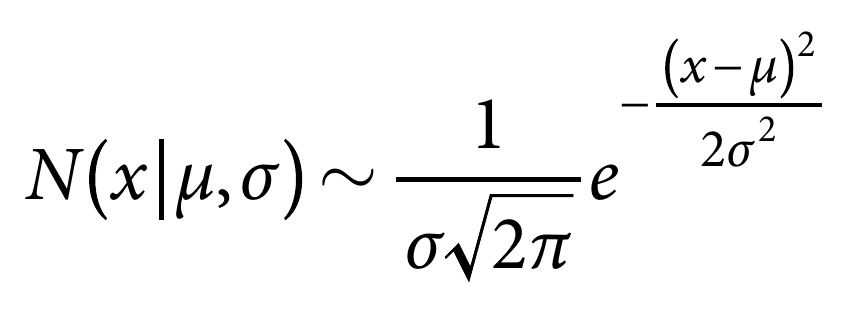
\includegraphics[width=0.40000\textwidth]{figs/9a-1.png}
\caption{the normal distribution}
\end{figure}

The parameter \(\mu\) is the mean and median

\begin{itemize}
\tightlist
\item
  and controls where the distribution is centered
\item
  (because this is a symmetric distribution),
\end{itemize}

and the parameter \(\sigma\) controls

\begin{itemize}
\tightlist
\item
  how spread out the distribution is.
\end{itemize}

Note the Greek letter parameters (estimators)

\begin{itemize}
\tightlist
\item
  and the Latin letters for data (variables)
\end{itemize}

This is the general functional form,

\begin{itemize}
\tightlist
\item
  but for specific real-world phenomenon,
\item
  these parameters have actual numbers as values,
\item
  which we can estimate from the data.
\end{itemize}

\paragraph{A bunch of distributions for different
uses}\label{a-bunch-of-distributions-for-different-uses}

\begin{figure}
\centering
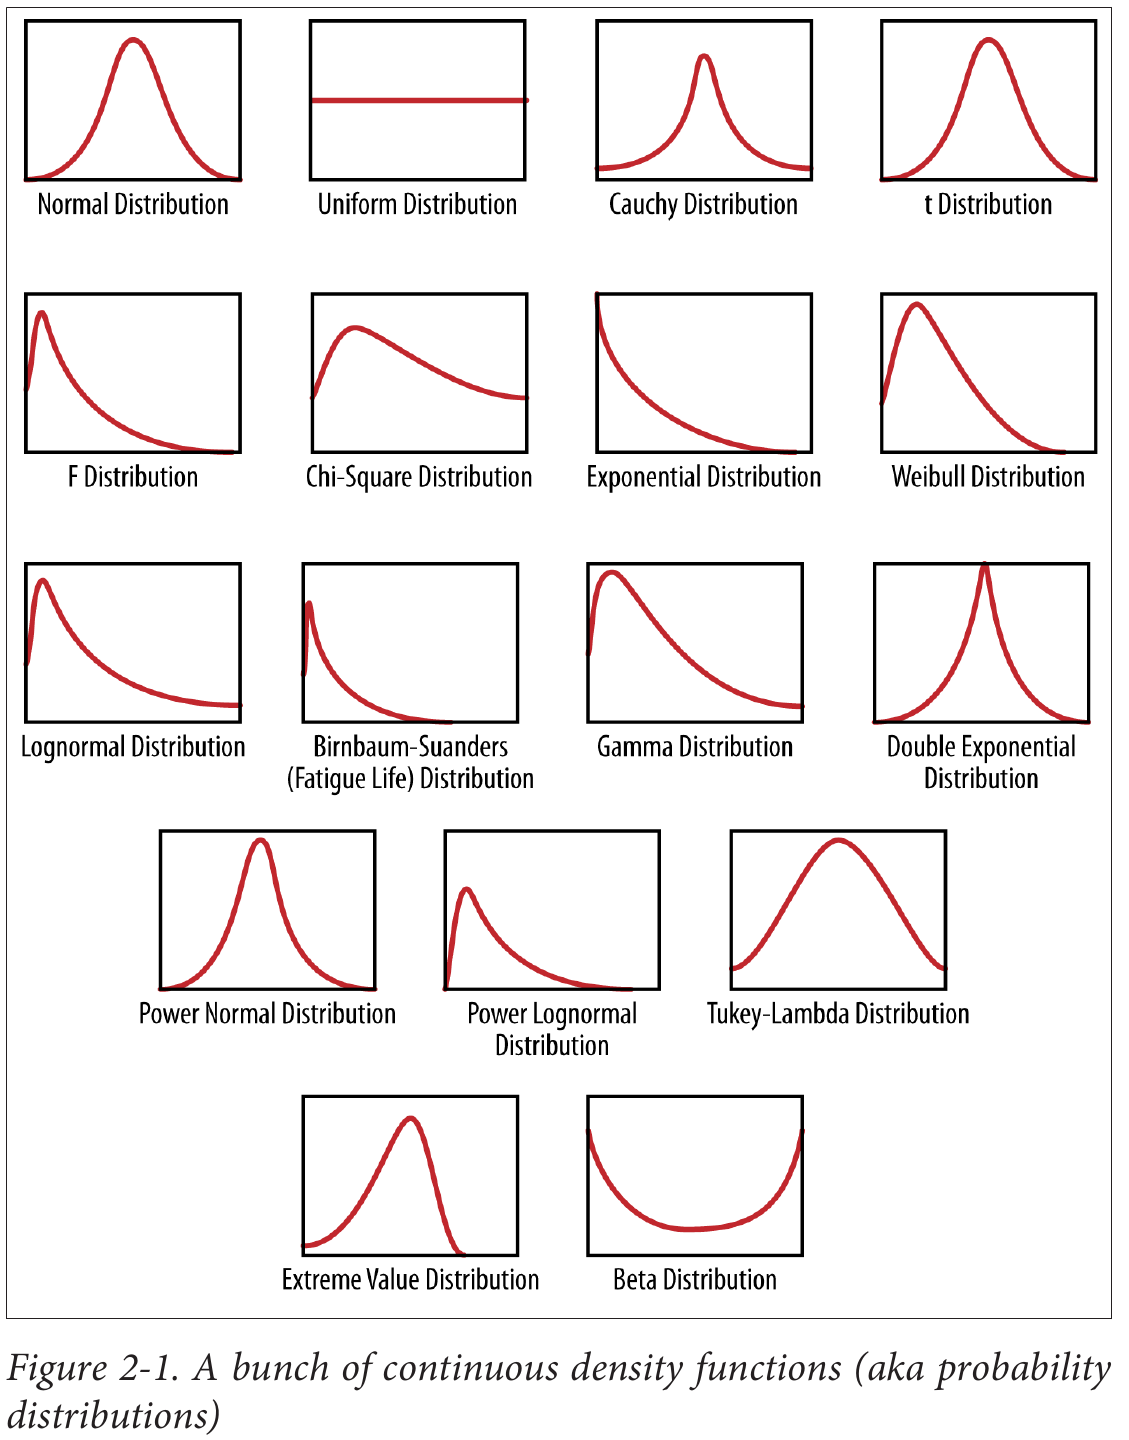
\includegraphics[width=0.70000\textwidth]{figs/9a-2.png}
\caption{distributions}
\end{figure}

\subparagraph{\texorpdfstring{Distribution of a single random variable
\(p(x)\)}{Distribution of a single random variable p(x)}}\label{distribution-of-a-single-random-variable-px}

A random variable denoted by x or y can be assumed to have

\begin{itemize}
\tightlist
\item
  a coresponding probability distribution, \(p(x)\) ,
\item
  which maps x to a positive real number.
\end{itemize}

In order to be a probability density function,

\begin{itemize}
\tightlist
\item
  we're restricted to the set of functions
\item
  such that if we integrate p (x) to get the area under the curve,
\item
  it is 1, so it can be interpreted as probability.
\end{itemize}

\subparagraph{\texorpdfstring{Joint distributions
\(p(x,y)\)}{Joint distributions p(x,y)}}\label{joint-distributions-pxy}

In addition to denoting distributions of single random variables

\begin{itemize}
\tightlist
\item
  with functions of one variable,
\end{itemize}

we use multivariate functions called joint distributions

\begin{itemize}
\tightlist
\item
  to do the same thing for more than one random variable.
\end{itemize}

So in the case of two random variables, for example,

\begin{itemize}
\tightlist
\item
  we could denote our distribution by a function p (x,y),
\item
  and it would take values in the plane
\item
  and give us nonnegative values.
\end{itemize}

In keeping with its interpretation as a probability,

\begin{itemize}
\tightlist
\item
  its (double) integral over the whole plane would be 1.
\end{itemize}

\subparagraph{\texorpdfstring{Conditional Distributions
\(p(x|y)\)}{Conditional Distributions p(x\textbar{}y)}}\label{conditional-distributions-pxy}

a conditional distribution, \(p(x|y)\)

\begin{itemize}
\tightlist
\item
  which is to be interpreted as
\item
  the density function of \(x\)
\item
  given a particular value of \(y\).
\end{itemize}

When we're working with data,

\begin{itemize}
\tightlist
\item
  conditioning corresponds to subsetting.
\item
  i.e.~applying a condition to the dataset
\end{itemize}

Example

\begin{itemize}
\tightlist
\item
  suppose we have a set of user-level data for Amazon.com
\item
  that lists for each user

  \begin{itemize}
  \tightlist
  \item
    the amount of money spent last month on Amazon,
  \item
    whether the user is male or female,
  \item
    and how many items they looked at before adding the first item to
    the shopping cart.
  \end{itemize}
\end{itemize}

If we consider x to be the random variable that represents the amount of
money spent,

\begin{itemize}
\tightlist
\item
  then we can look at the distribution of money spent across all users,
\item
  and represent it as \(p(x)\).
\end{itemize}

We can then take the subset of users

\begin{itemize}
\tightlist
\item
  who looked at more than five items before buying anything,
\item
  and look at the distribution of money pent among these users.
\end{itemize}

Let y be the random variable that represents number of items looked at,

\begin{itemize}
\tightlist
\item
  then \(p(x|y) > 5\) would be the corresponding conditional
  distribution.
\end{itemize}

Note a conditional distribution has the same properties

\begin{itemize}
\tightlist
\item
  as a regular distribution in that
\item
  when we integrate it, it sums to 1 and has to take nonnegative values.
\end{itemize}

\paragraph{Fitting a model}\label{fitting-a-model}

Fitting a model means that

\begin{itemize}
\tightlist
\item
  you estimate the parameters of the model
\item
  using the observed data.
\end{itemize}

You are using your data as evidence to help approximate the real-world
mathematical process that generated the data.

Fitting the model often involves optimization methods and algorithms,

\begin{itemize}
\tightlist
\item
  such as maximum likelihood estimation,
\item
  to help get the parameters.
\end{itemize}

In fact, when you estimate the parameters,

\begin{itemize}
\tightlist
\item
  they are actually estimators,
\item
  meaning they themselves are functions of the data.
\end{itemize}

Once you fit the model, you actually can write it as y = 7.2 + 4.5x, for
example, which means that your best guess is that this equation or
functional form expresses the relationship between your two variables,
based on your assumption that the data followed a linear pattern.

Beware of overfitting

\begin{itemize}
\tightlist
\item
  The Bias-Variance Tradeoff
\item
  \url{https://en.wikipedia.org/wiki/Bias\%E2\%80\%93variance_tradeoff}

  \begin{itemize}
  \tightlist
  \item
    More discussed in DSCI353-453
  \item
    And in Introduction to Statistical Learning with R (ISLR book)
  \end{itemize}
\end{itemize}

\paragraph{Exploratory Data Analysis}\label{exploratory-data-analysis}

``Exploratory data analysis'' is an attitude, a state of flexibility, a
willingness to look for those things that we believe are not there, as
well as those we believe to be there.

--- John Tukey

John Tukey, a mathematician at Bell Labs, - developed exploratory data
analysis in contrast to confirmatory data analysis, - which concerns
itself with modeling and hypotheses.

In EDA, there is no hypothesis and there is no model. - The
``exploratory'' aspect means that - your understanding of the problem
you are solving, or might solve, - is changing as you go.

The basic tools of EDA are plots, graphs and summary statistics.

Generally speaking, it's a method of systematically going through the
data,

\begin{itemize}
\tightlist
\item
  plotting distributions of all variables (using box plots),
\item
  plotting time series of data,
\item
  transforming variables,
\item
  looking at all pairwise relationships between variables

  \begin{itemize}
  \tightlist
  \item
    using scatterplot matrices,
  \end{itemize}
\item
  and generating summary statistics for all of them.
\end{itemize}

At the very least that would mean

\begin{itemize}
\tightlist
\item
  computing their mean,
\item
  minimum,
\item
  maximum,
\item
  the upper and lower quartiles,
\item
  and identifying outliers.
\end{itemize}

\subparagraph{Philosophy of Exploratory Data
Analysis}\label{philosophy-of-exploratory-data-analysis}

Long before worrying about how to convince others, you first have to
understand what's happening yourself.

--- Andrew Gelman

\paragraph{The Data Science Process}\label{the-data-science-process}

Let's put it all together into what we define as the data science
process.

\begin{figure}
\centering
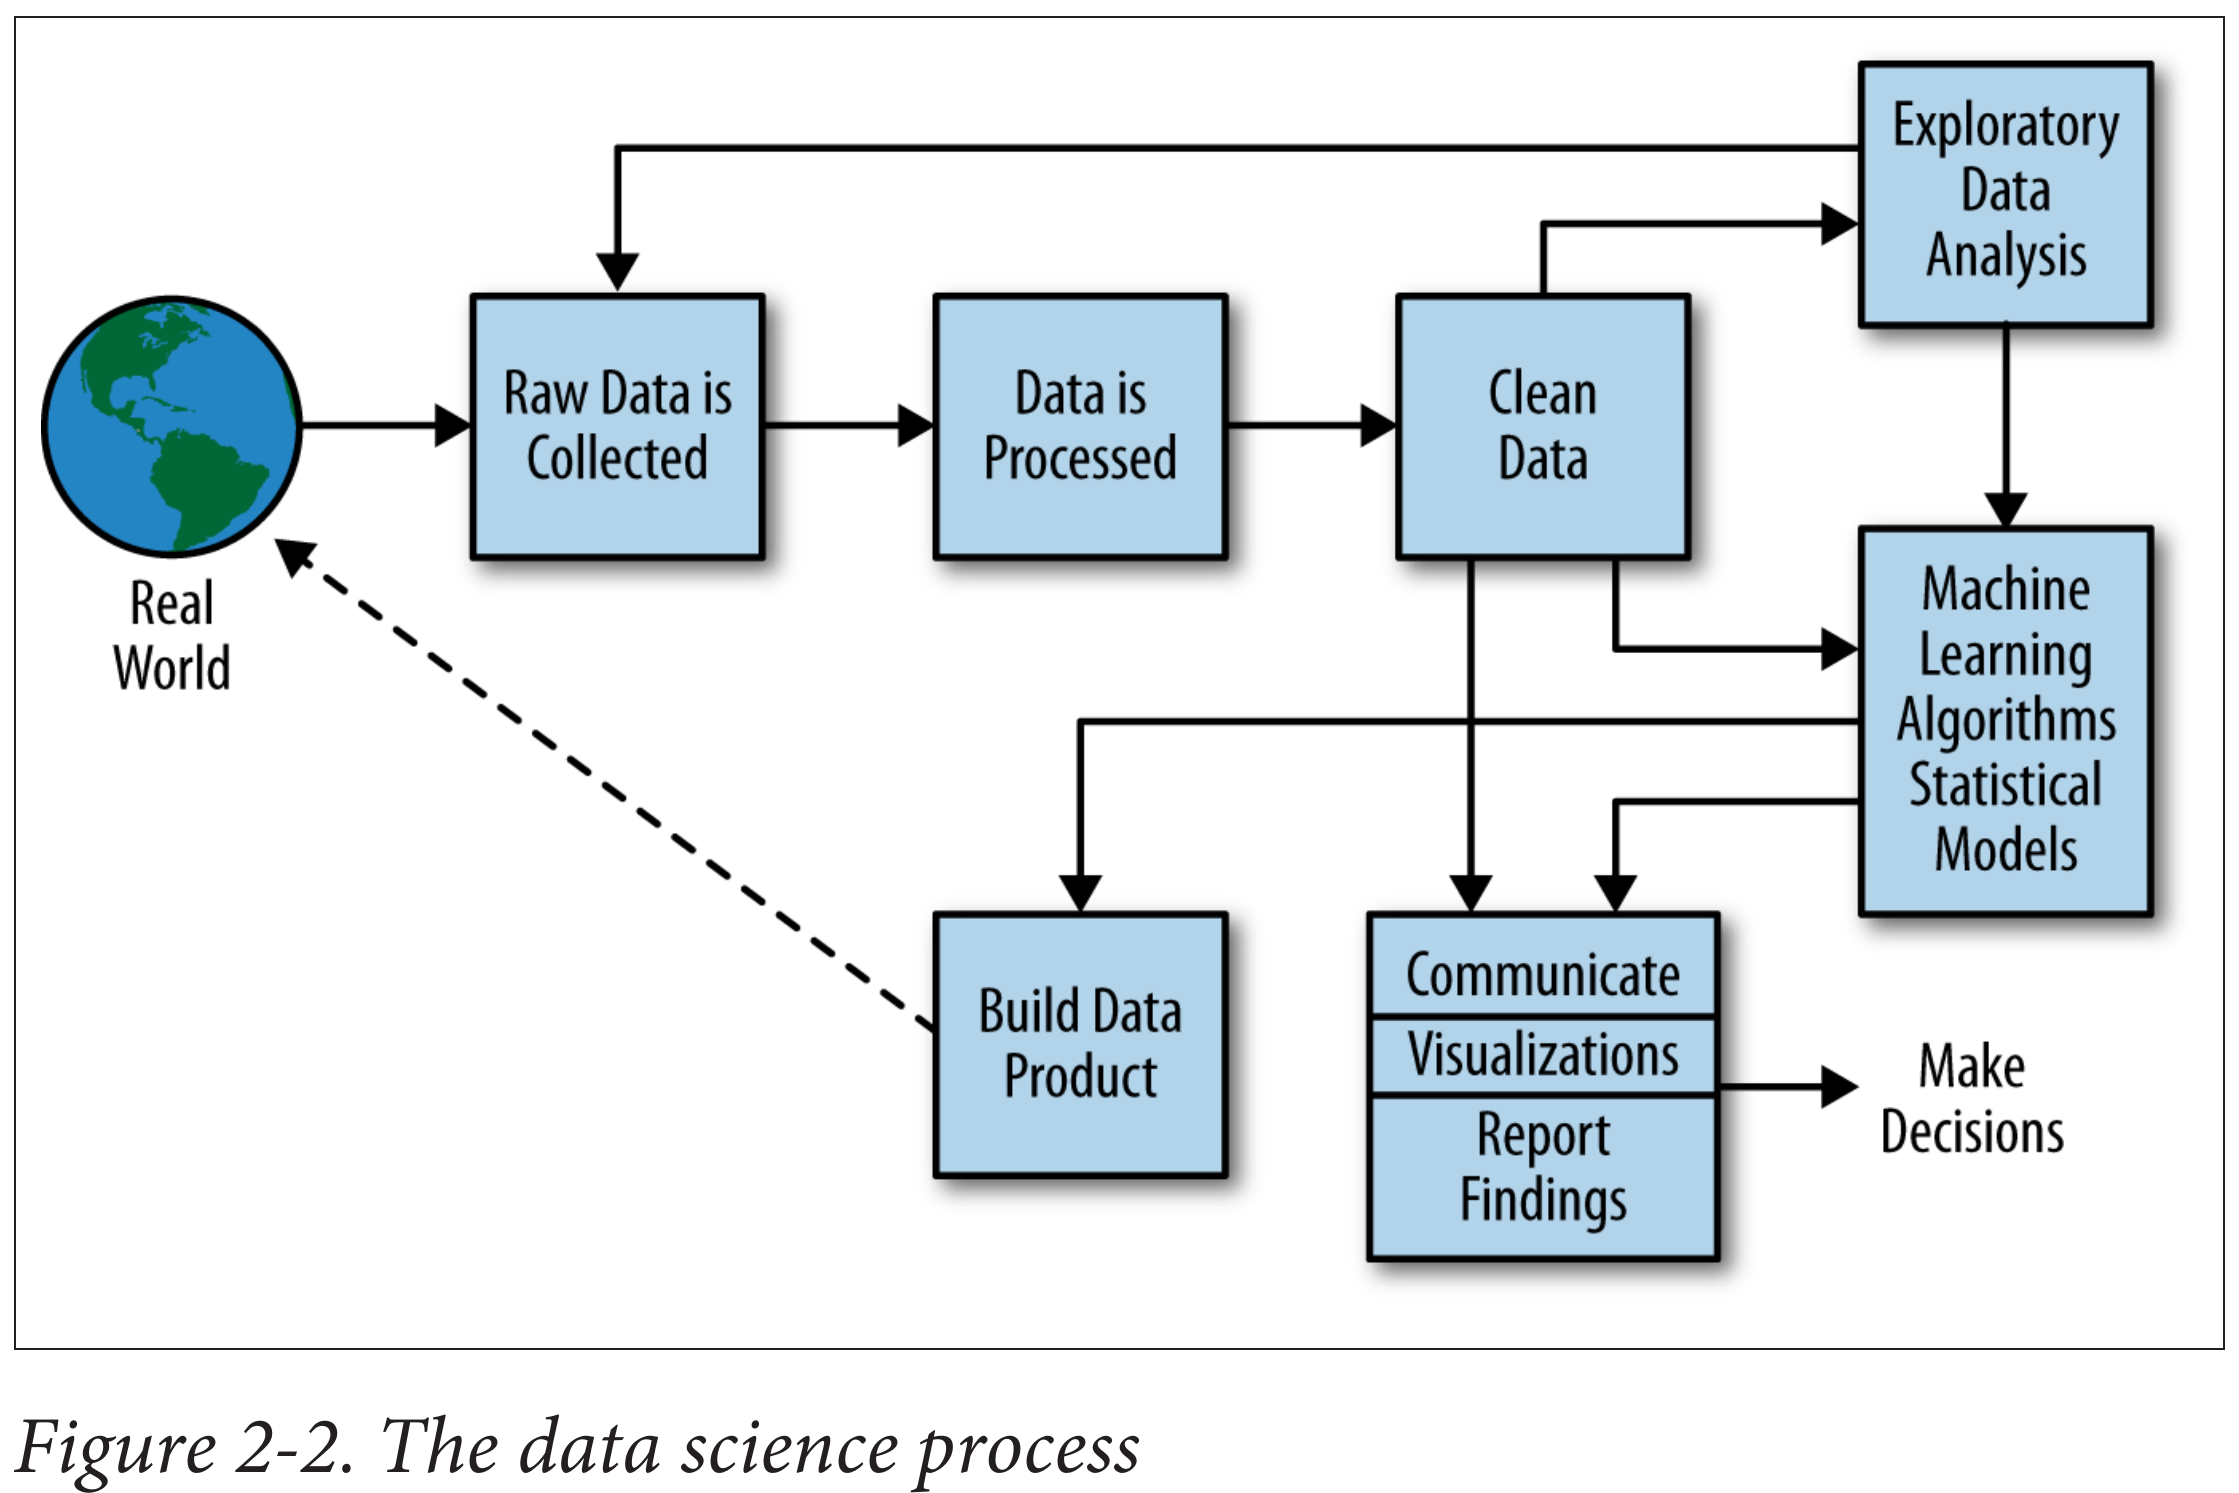
\includegraphics[width=0.70000\textwidth]{figs/9a-3.png}
\caption{the data science process}
\end{figure}

First we have the Real World.

Inside the Real World are lots of people busy at various activities.

We start with raw data

We want to process this to make it clean for analysis. So we build and
use pipelines of data munging: joining, scraping, wrangling, or whatever
you want to call it. To do this we use tools such as Python, shell
scripts, R, or SQL, or all of the above.

Once we have this clean dataset,

\begin{itemize}
\tightlist
\item
  we should be doing some kind of EDA.
\end{itemize}

In the course of doing EDA, we may realize

\begin{itemize}
\tightlist
\item
  that it isn't actually clean because of

  \begin{itemize}
  \tightlist
  \item
    duplicates, missing values, absurd outliers,
  \item
    and data that wasn't actually logged or incorrectly logged.
  \end{itemize}
\end{itemize}

If that's the case, we may have to go back

\begin{itemize}
\tightlist
\item
  to collect more data,
\item
  or spend more time cleaning the dataset.
\end{itemize}

Next, we design our model to use some algorithm

\begin{itemize}
\tightlist
\item
  like k-nearest neighbor (k-NN), linear regression, Naive Bayes, or
  something else.
\end{itemize}

The model we choose depends on the type of problem we're trying to
solve,

\begin{itemize}
\tightlist
\item
  The type of data science problem/question could be
\item
  a classification problem,
\item
  a prediction problem,
\item
  or a basic description problem.
\end{itemize}

\paragraph{A Data Scientist's Role in This
Process}\label{a-data-scientists-role-in-this-process}

\begin{figure}
\centering
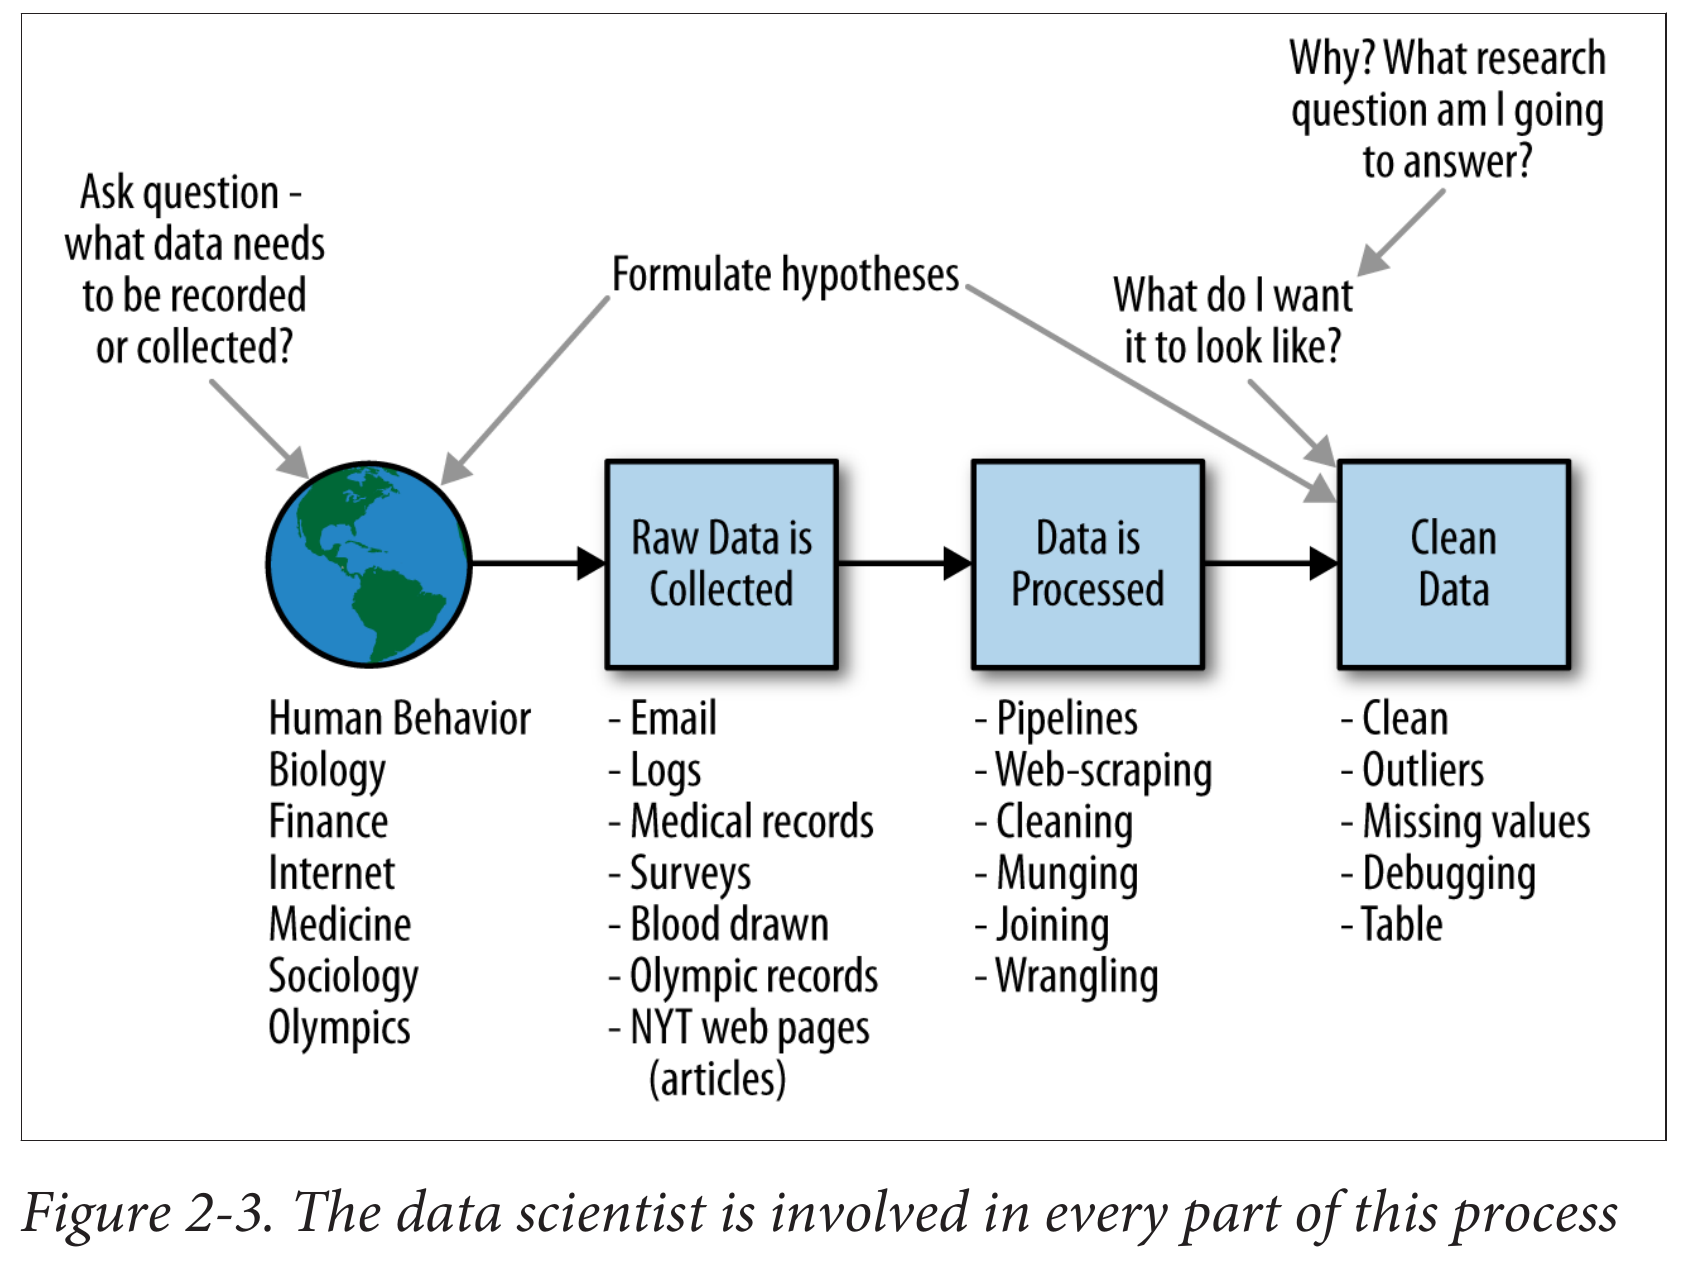
\includegraphics[width=0.70000\textwidth]{figs/9a-4.png}
\caption{the role of thedata scientist}
\end{figure}


\end{document}
